\documentclass{article}
\usepackage[utf8]{inputenc}
\usepackage{titling}
\usepackage{lipsum}
\usepackage[space]{grffile}
%\usepackage{natbib}
\usepackage{graphicx}
\usepackage{url}
\usepackage{amsmath}
\usepackage{amssymb}

\usepackage{float}

\voffset=-1.0in
\hoffset=-0.5in
\textheight 9.0truein
\textwidth 6.0truein




\newcommand{\figwid}{0.9\linewidth}

\title{\bf Access-Optimized Priority Search Tree}
\author{\Large {Haley Massa} and {Jeffrey Uhlmann} \\
Dept.\ of Electrical Engineering and Computer Science\\
University of Missouri - Columbia}
\date{}


\begin{document}

\maketitle

\begin{abstract}
In this paper we show that the priority search tree of McCreight, which was originally developed to satisfy a class of spatial search queries on 2-dimensional points, can be applied to the problem of dynamically maintaining a set of keys so that the query complexity adapts to the distribution of queried keys. Presently, the best-known example of such a data structure is the splay tree, which dynamically reconfigures itself during each query so that frequently accessed keys move to the top of the tree and thus can be retrieved with fewer queries than keys that are lower in the tree. However, while the splay tree is conjectured to offer optimal adaptive amortized query complexity, it may require $O(n)$ for individual queries. We show that an access-optimized priority search tree (AOPST) can provide competitive adaptive query performance while ensuring $O(\log n)$ worst-case query performance, thus potentially making it more suitable for certain interactive (e.g.,online and real-time) applications for which the response time must be bounded.  
\end{abstract}

\section{Introduction}

Many applications demand the efficient satisfaction of key-retrieval queries from a dynamically-maintained search structure (database) of $n$ keys. In many of these applications certain keys are queried much more frequently than other keys, and this nonuniform sampling from the set of $n$ keys can potentially be exploited by a distribution-sensitive search structure to surpass the $O(\log n)$ comparison-based theoretical lower bound on the expected number of comparisons per query required in the uniform case. 

The splay tree, developed by Daniel Sleator and Robert Tarjan \cite{splay}, is a self-adjusting \cite{selfadj} binary search tree that optimizes its structure to the distribution patterns of the dataset. Splay trees differ from standard balanced BSTs by performing rotations that migrate frequently-accessed keys to the top of the tree so that the search paths to those keys will be shorter when accessed during future queries. A novelty of the splay tree is that it does not necessarily enforce balance at all times during a given sequence of $n$ updates and/or queries, but it does guarantee that the complexity of any given sequence is $O(n\log n)$. The value of the splay tree as an access-sensitive search structure is that it can offer sequence time complexity approaching $O(n)$ if the access distribution of keys is highly nonuniform. By contrast, a standard balanced BST (e.g., AVL, red-black, etc. \cite{bst}) provides no access-distribution sensitivity and thus can be expected to require $O(n \log n)$ time to perform a sequence of $O(n)$ operations. A natural question is whether it is possible to combine the access-sensitive properties of the splay tree with the efficient worst-case properties of a balanced BST. 

In this paper we show that the {\em priority search tree} \cite{pst}, which was published in the same year as the splay tree (1985), can be applied to achieve adaptive query performance that is competitive with the splay tree while providing superior worst-case optimal $O(\log n)$ update and query complexity. This {\em access-optimized} priority search tree (AOPST) is described in the following section. We then provide practical comparisons of the AOPST and splay tree in the form of simulation results with varying degrees of nonuniformity in the sampling of query keys.


\section{Adaptive Priority Search Tree}

The {\em priority search tree} (PST) is a data structure introduced by Edward McCreight in 1985 with the objective of storing a set of $n$ points in $\mathbb{R}^2$ in a way that allows for $O(\log n)$ update complexity, i.e., insertion or deletion of a point, and $O(\log n + k)$ complexity for semi-infinite 2-dimensional range queries where $k$ is the number of returned objects. This complexity is achieved by maintaining the points simultaneously in BST order on the $x$ coordinates and heap order on the $y$ coordinates within the same binary tree structure. The data structure allows for five main operations on a dataset $D$ of ordered pairs to be performed efficiently:
\begin{enumerate}
\item Insert an ordered pair into $D$.
\item Delete an ordered pair from $D$.
\item Given integers $x_0$, $x1$, and $y1$, among all the pairs $(x, y)$ in $D$ such that $x_0 \leq x \leq x_1$ and $y \leq y_1$, find the pair whose $x$ is minimal.
\item Given integers $x_0$ and $x_1$, among all the pairs $(x, y)$ in $D$ such that $x_0 \leq x \leq x_1$, find the pair whose $y$ is minimal.
\item Given integers $x_0$, $x_1$, and $y_1$, enumerate all $k$ pairs $(x, y)$ in $D$ such that $x_0 \leq x \leq x_1$ and $y \leq y_1$.
\end{enumerate}
The priority search tree was the first data structure to support 2-dimensional spatial search queries within the same $O(\log n + k)$ complexity of 1-dimensional range queries offered by balanced binary search trees (BSTs) while also supporting $O(\log n)$ update operations. Specifically operations 1-4 have time complexity $O(\log n)$ and operation 5 has $O(\log n + k)$ complexity. 

Each node in a priority search tree contains exactly one ordered pair $(x, y)$. A maximum PST is constructed so that the $y$-value of every child node is less than or equal to that of its parent whereas in a minimum PST the $y$-value of a child node is greater than or equal to it parent's $y$-value. In both cases, the $x$-value of every node in a right subtree is strictly less than that of every node in the left subtree. Furthermore, the cardinality of a node’s right subtree is equal to or one less than the node’s left subtree, ensuring balance.  

While the priority search tree was originally created to store two-dimensional coordinates, we introduce here an alternative use of the data structure. With some slight construction and operation alterations, the priority search tree can be used as a distribution-sensitive search structure. We will call this specialized structure an {\em access optimized priority search tree} (AOPST). The AOPST stores each key of a dataset in the x-value of a node and its respective access frequency as the y-value. In other words, the skeleton of the tree maintains a BST ordering of the keys while the access-freqencies associated with the keys are maintained in heap order. By slightly altering the search algorithms of a regular priority search tree, any search key can be found (or not found) in an AOPST in $O(\log n)$ time. The principal change to the standard PST is the incrementing of the priorities (access frequencies) associated with the keys. Specifically, when a key is accessed by either an update or a query, its access count is incremented and the key's position in the heap may then also be incremented.

\section{Comparative Performance Results}

In this section we examine the relative performance characteristics of a conventional balanced binary search tree (BST), a splay tree, and the AOPST. In the case of uniformly sampled query keys, the splay tree and AOPST incur extra overhead compared to the BST. In the case of the splay tree, this overhead takes the form of extra comparisons performed as the tree is restructured. In the case of the AOPST, the overhead takes the form of an extra key comparison per node visited: one comparison to the key stored at each node according to heap order, and another comparison to the pivot key stored at each node for use in traversing the tree according to BST order. Therefore, the goal of our tests is to examine how relative number of key comparisons used during the search of each data structure is affected by the distribution of queried keys. We should expect the BST to be superior in the uniform case while the splay tree and AOPST should perform better as the distribution becomes increasingly nonuniform. 

We define a value $p$, $0\leq p\leq 1$, to parameterize our key-access testing distributions with $p=0$ representing a uniform random distribution of key accesses; $p=1$ representing an exponentially-distributed sequence of accesses with the most frequently-accessed key representing approximately $50\%$ of the accesses, the next representing $25\%$ of the accesses, etc., such that $O(\log n)$ of the keys comprise $O(n)$ of the accesses; and $0<p<1$ representing a weighted mixture of accesses from the two distributions. 
	
As can be seen in Figure \ref{fig:p-0}, the splay and AOPS trees perform comparably but are outperformed by the BST because of its lower overhead. In other words, the overhead of adaptivity incurred by the splay and AOPS trees does not yield dividends in the case of keys that are queried uniform-randomly. Figure \ref{fig:p-25} shows that the relative performance advantage of the BST decreases when $25\%$ of the key accesses exponentially distributed access frequencies. Figure \ref{fig:p-5} shows that when there is an equal mix of keys sampled from the uniform and exponential distributions the three search structures perform comparably. In the case of all keys sampled exponentially, Figures \ref{fig:p-75} and \ref{fig:p-1} show that the distribution-sensitivity properties of the splay and AOPS trees provide a significant performance advantage over the BST as the access frequencies tend toward an exponential distribution.

\begin{figure}[H]
\begin{center}
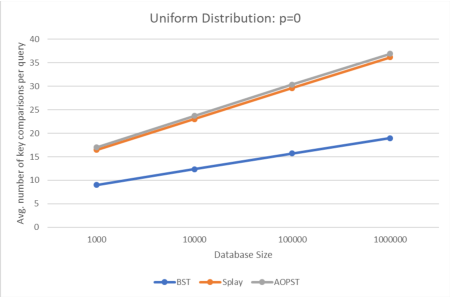
\includegraphics[width=\figwid,keepaspectratio]{p-0.pdf}
\caption{\footnotesize This figure shows the average number of key comparisons for query keys drawn from uniform distribution for datasets of increasing size $n$. The expected number of key comparisons performed by the BST is $\log(n)$ while the splay and AOPS trees perform roughly twice as many comparisons per query.}
\label{fig:p-0}
\end{center}
\end{figure}

\begin{figure}[H]
\begin{center}
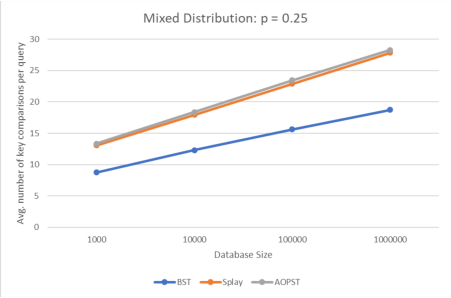
\includegraphics[width=\figwid,keepaspectratio]{p-25.pdf}
\caption{\footnotesize This figure shows the average number of key comparisons when the $1/4$ of the query keys are sampled with exponential frequency and the remaining are sampled uniformly.}
\label{fig:p-25}
\end{center}
\end{figure}

\begin{figure}[H]
\begin{center}
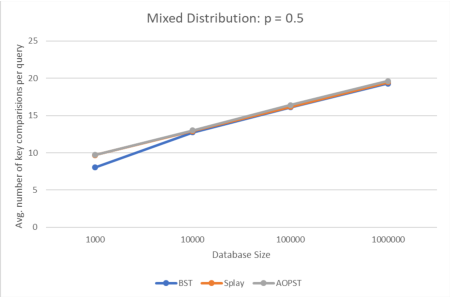
\includegraphics[width=\figwid,keepaspectratio]{p-5.pdf}
\caption{\footnotesize This figure shows the average number of key comparisons when half of the query keys are sampled with exponential frequency and the remaining half are sampled uniformly.}
\label{fig:p-5}
\end{center}
\end{figure}


\begin{figure}[H]
\begin{center}
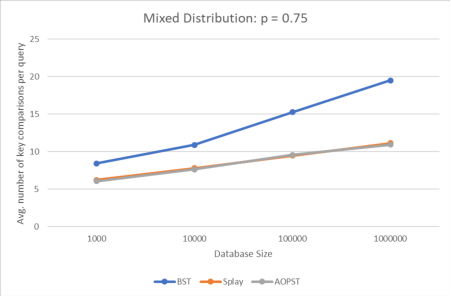
\includegraphics[width=\figwid,keepaspectratio]{p-75.pdf}
\caption{\footnotesize This figure shows the average number of key comparisons when $75\%$ of the query keys are sampled according to an exponetial distribution.}
\label{fig:p-75}
\end{center}
\end{figure}

\begin{figure}[H]
\begin{center}
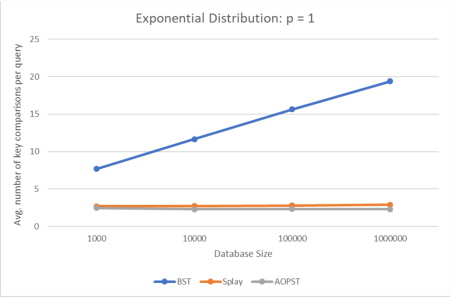
\includegraphics[width=\figwid,keepaspectratio]{p-1.pdf}
\caption{\footnotesize This figure shows the average number of key comparisons when all query keys are sampled according to an exponential distribution, i.e., the frequency of access of different keys decreases exponentially.}
\label{fig:p-1}
\end{center}
\end{figure}


\section{Discussion}

The principal contribution of this paper is the demonstration that the classical priority search tree of McCreight can be reinterpreted so that instead of storing 2-dimensional points it is adapted for the access-sensitive storage and retrieval of 1-dimensional keys. As can be seen from the test results, the access-optimized priority search tree offers comparable access-sensitive performance to the splay tree while bounding the complexity of each operation, a property which is needed for interactive applications that must impose strict constraints on the worst-case response time of each operation.  



\bibliographystyle{plain}
\begin{thebibliography}{9}

\bibitem{selfadj}
B.\ Allen and I.\ Munro, ``Self-organizing search trees,'' {\em Journal of the ACM}, 25 (4): 526–535, 1978.

\bibitem{pst}
McCreight, Edward, ``Priority search trees,'' {\em SIAM Journal on Scientific Computing}, 14 (2): 257–276, 1985.

\bibitem{bst}
Sedgewick, Robert, ``Balanced Trees,'' {\em Algorithms}, Addison-Wesley, 1983.

\bibitem{splay}
Sleator, Daniel D.; Tarjan, Robert E., ``Self-Adjusting Binary Search Trees,'' {\em Journal of the ACM}, 32 (3): 652–686. 1985.

\end{thebibliography}



\end{document}